\documentclass[journal,12pt,twocolumn]{IEEEtran}
%
\makeatletter
\makeatother
\usepackage{setspace}
\usepackage{gensymb}
\usepackage{xcolor}
\usepackage{caption}
%\usepackage{stackengine}
%\usepackage{subcaption}
%\doublespacing
\singlespacing



\usepackage{graphicx}
\graphicspath{ {./images}  }
%\usepackage{amssymb}
%\usepackage{relsize}
\usepackage[cmex10]{amsmath}
\usepackage{mathtools}
%\usepackage{amsthm}
\interdisplaylinepenalty=2500
%\savesymbol{iint}
%\usepackage{txfonts}
%\restoresymbol{TXF}{iint}
\usepackage{wasysym}
\usepackage{amsthm}
\usepackage{mathrsfs}
\usepackage{txfonts}
\usepackage{stfloats}
\usepackage{cite}
\usepackage{cases}
\usepackage{mathtools}
\usepackage{subfig}
\usepackage{enumerate}	
\usepackage{enumitem}
\usepackage{amsmath}
%\usepackage{xtab}
\usepackage{longtable}
\usepackage{multirow}
%\usepackage{algorithm}
%\usepackage{algpseudocode}
\usepackage{enumitem}
\usepackage{mathtools}
%\usepackage{iithtlc}
\usepackage{tikz}
\usetikzlibrary{shapes,arrows}
%\usetikzlibrary{arrows.meta,calc,positioning}
%\usepackage[framemethod=tikz]{mdframed}
\usepackage{listings}
    \usepackage[latin1]{inputenc}                                 %%
    \usepackage{color}                                            %%
    \usepackage{array}                                            %%
    \usepackage{longtable}                                        %%
    \usepackage{calc}                                             %%
    \usepackage{multirow}                                         %%
    \usepackage{hhline}                                           %%
    \usepackage{ifthen}                                           %%
  %optionally (for landscape tables embedded in another document): %%
    \usepackage{lscape}     



%\usepackage{stmaryrd}


%\usepackage{wasysym}
%\newcounter{MYtempeqncnt}
\DeclareMathOperator*{\Res}{Res}
%\renewcommand{\baselinestretch}{4}
%\setcounter{secnumdepth}{4}
\renewcommand\thesection{\arabic{section}}
\renewcommand\thesubsection{\thesection.\arabic{subsection}}
\renewcommand\thesubsubsection{\thesubsection.\arabic{subsubsection}}
%\renewcommand\thesubsubsubsection{\thesubsubsection.\arabic{subsubsubsection}}

%\renewcommand\thesectiondis{\arabic{section}}
%\renewcommand\thesubsectiondis{\thesectiondis.\arabic{subsection}}
%\renewcommand\thesubsubsectiondis{\thesubsectiondis.\arabic{subsubsection}}
%\renewcommand\thesubsubsubsectiondis{\thesubsubsectiondis.\arabic{subsubsubsection}}
% correct bad hyphenation here
\hyphenation{op-tical net-works semi-conduc-tor}

%\lstset{
%language=C,
%frame=single, 
%breaklines=true
%}

%\lstset{
	%%basicstyle=\small\ttfamily\bfseries,
	%%numberstyle=\small\ttfamily,
	%language=Octave,
	%backgroundcolor=\color{white},
	%%frame=single,
	%%keywordstyle=\bfseries,
	%%breaklines=true,
	%%showstringspaces=false,
	%%xleftmargin=-10mm,
	%%aboveskip=-1mm,
	%%belowskip=0mm
%}

%\surroundwithmdframed[width=\columnwidth]{lstlisting}
\def\inputGnumericTable{}                                 %%

\lstset{
%language=python,
frame=single, 
breaklines=true,
columns=fullflexible
}

 

\begin{document}
%
\tikzstyle{block} = [rectangle, draw,
text width=7em, text centered, minimum height=4em]
\tikzstyle{sum} = [draw, circle, node distance=3cm]
\tikzstyle{input} = [coordinate]
\tikzstyle{output} = [coordinate]
\tikzstyle{pinstyle} = [pin edge={to-,thin,black}]
\tikzstyle{line} = [draw, -latex']
\theoremstyle{definition}
\newtheorem{theorem}{Theorem}[section]
\newtheorem{problem}{Problem}
\newtheorem{proposition}{Proposition}[section]
\newtheorem{lemma}{Lemma}[section]
\newtheorem{corollary}[theorem]{Corollary}
\newtheorem{example}{Example}[section]
\newtheorem{definition}{Definition}[section]
%\newtheorem{algorithm}{Algorithm}[section]
%\newtheorem{cor}{Corollary}
\newcommand{\BEQA}{\begin{eqnarray}}
\newcommand{\EEQA}{\end{eqnarray}}
\newcommand{\define}{\stackrel{\triangle}{=}}

\bibliographystyle{IEEEtran}
%\bibliographystyle{ieeetr}

\providecommand{\nCr}[2]{\,^{#1}C_{#2}} % nCr
\providecommand{\nPr}[2]{\,^{#1}P_{#2}} % nPr
\providecommand{\mbf}{\mathbf}
\providecommand{\pr}[1]{\ensuremath{\Pr\left(#1\right)}}
\providecommand{\qfunc}[1]{\ensuremath{Q\left(#1\right)}}
\providecommand{\sbrak}[1]{\ensuremath{{}\left[#1\right]}}
\providecommand{\lsbrak}[1]{\ensuremath{{}\left[#1\right.}}
\providecommand{\rsbrak}[1]{\ensuremath{{}\left.#1\right]}}
\providecommand{\brak}[1]{\ensuremath{\left(#1\right)}}
\providecommand{\lbrak}[1]{\ensuremath{\left(#1\right.}}
\providecommand{\rbrak}[1]{\ensuremath{\left.#1\right)}}
\providecommand{\cbrak}[1]{\ensuremath{\left\{#1\right\}}}
\providecommand{\lcbrak}[1]{\ensuremath{\left\{#1\right.}}
\providecommand{\rcbrak}[1]{\ensuremath{\left.#1\right\}}}
\theoremstyle{remark}
\newtheorem{rem}{Remark}
\newcommand{\sgn}{\mathop{\mathrm{sgn}}}
\providecommand{\abs}[1]{\left\vert#1\right\vert}
\providecommand{\res}[1]{\Res\displaylimits_{#1}} 
\providecommand{\norm}[1]{\lVert#1\rVert}
\providecommand{\mtx}[1]{\mathbf{#1}}
\providecommand{\mean}[1]{E\left[ #1 \right]}
\providecommand{\fourier}{\overset{\mathcal{F}}{ \rightleftharpoons}}
%\providecommand{\hilbert}{\overset{\mathcal{H}}{ \rightleftharpoons}}
\providecommand{\system}{\overset{\mathcal{H}}{ \longleftrightarrow}}
	%\newcommand{\solution}[2]{\textbf{Solution:}{#1}}
\newcommand{\solution}{\noindent \textbf{Solution: }}
\providecommand{\dec}[2]{\ensuremath{\overset{#1}{\underset{#2}{\gtrless}}}}
\DeclarePairedDelimiter{\ceil}{\lceil}{\rceil}
%\numberwithin{equation}{subsection}
\numberwithin{equation}{section}
%\numberwithin{problem}{subsection}
%\numberwithin{definition}{subsection}
%\makeatletter
%\@addtoreset{figure}{section}
%\makeatother

\let\StandardTheFigure\thefigure
%\renewcommand{\thefigure}{\theproblem.\arabic{figure}}
%\renewcommand{\thefigure}{\thesection}


%\numberwithin{figure}{subsection}

%\numberwithin{equation}{subsection}
%\numberwithin{equation}{section}
%\numberwithin{equation}{problem}
%\numberwithin{problem}{subsection}
%\numberwithin{problem}{section}
%%\numberwithin{definition}{subsection}
%\makeatletter
%\@addtoreset{figure}{problem}
%\makeatother
%\makeatletter
%\@addtoreset{table}{problem}
%\makeatother

\let\StandardTheFigure\thefigure
\let\StandardTheTable\thetable
%%\renewcommand{\thefigure}{\theproblem.\arabic{figure}}
%\renewcommand{\thefigure}{\theproblem}

%%\numberwithin{figure}{section}

%%\numberwithin{figure}{subsection}



\def\putbox#1#2#3{\makebox[0in][l]{\makebox[#1][l]{}\raisebox{\baselineskip}[0in][0in]{\raisebox{#2}[0in][0in]{#3}}}}
     \def\rightbox#1{\makebox[0in][r]{#1}}
     \def\centbox#1{\makebox[0in]{#1}}
     \def\topbox#1{\raisebox{-\baselineskip}[0in][0in]{#1}}
     \def\midbox#1{\raisebox{-0.5\baselineskip}[0in][0in]{#1}}




\title{ 
%	\logo{
Implementation of Low Density Parity Check (LDPC) codes
%	}
}



\author{Theresh Babu Benguluri, Sandeep Kumar Khyalia and G V V Sharma$^{*}$% <-this % stops a space
\thanks{*The author is with the Department
of Electrical Engineering, Indian Institute of Technology, Hyderabad
502285 India e-mail:  gadepall@iith.ac.in.}
}


% make the title area
\maketitle

\tableofcontents

%\bigskip
%
\begin{abstract}
\boldmath
A brief description about the design and implementataion of LDPC codes using (7,4) Hamming parity check matrix.
\end{abstract}


%\IEEEpeerreviewmaketitle

\section{Introduction}
Let the Channel model be,
\begin{equation}
Y_k= X_k + V_k, \quad k = 0,\dots,6
\end{equation} 
where $X_k$ is the  transmitted symbol in the $k$th time slot using the BPSK modulation and $V_k(m) \sim \mathcal{N}\brak{0,\sigma^2} $. 

\section{Encoding}
 LDPC codes are popular linear block codes with closest shannon limt channel capacity \cite{ldpc}. As an example Lets take (7,4) Hamming parity check matrix.
 \begin{equation} \label{eq:H}
 H =  \begin{bmatrix} 
1 & 1 & 1 & 0 & 1 & 0 & 0 \\
1 & 0 & 1 & 1 & 0 & 1 & 0 \\
1 & 1 & 0 & 1 & 0 & 0 & 1 
\end{bmatrix}
 \end{equation}

Above $H$ matrix having the parameters, information bits $k=4$ i.e $m=m_0,\dots,m_3$ , parity bits are $m=n-k=3$ i.e $p=[p_0,p_1,p_2]$ and  code word length $n=7$ i.e $c=[m\hspace{1mm}p]$.
\begin{figure}[!ht]
\begin{center}
%\begin{tikzpicture}
%
%    \node[shape=circle,draw=black] (v6) at (0,0) {v6};
%    \node[shape=circle,draw=black] (v5) at (0,1) {v5};
%    \node[shape=circle,draw=black] (v4) at (0,2) {v4};
%    \node[shape=circle,draw=black] (v3) at (0,3) {v3};
%    \node[shape=circle,draw=black] (v2) at (0,4) {v2};
%    \node[shape=circle,draw=black] (v1) at (0,5) {v1};
%    \node[shape=circle,draw=black] (v0) at (0,6) {v0};
%
%    
%
%
%    \node[shape=rectangle,draw=black] (p0) at (4,5) {p0};
%    \node[shape=rectangle,draw=black] (p1) at (4,3) {p1};
%    \node[shape=rectangle,draw=black] (p2) at (4,1) {p2};
%
%\path [-] (v0) edge node[left] {} (p0);
%\path [-] (v0) edge node[left] {} (p1);
%\path [-] (v0) edge node[left] {} (p2);
%\path [-] (v1) edge node[left] {} (p0);
%\path [-] (v1) edge node[left] {} (p2);
%\path [-] (v2) edge node[left] {} (p0);
%\path [-] (v2) edge node[left] {} (p1);
%\path [-] (v3) edge node[left] {} (p1);
%\path [-] (v3) edge node[left] {} (p2);
%\path [-] (v4) edge node[left] {} (p0);
%\path [-] (v5) edge node[left] {} (p1);
%\path [-] (v6) edge node[left] {} (p2);
%
%\path [->] (-1,0) edge node[left] {} (v6);
%\path [->] (-1,1) edge node[left] {} (v5);
%\path [->] (-1,2) edge node[left] {} (v4);
%\path [->] (-1,3) edge node[left] {} (v3);
%\path [->] (-1,4) edge node[left] {} (v2);
%\path [->] (-1,5) edge node[left] {} (v1);
%\path [->] (-1,6) edge node[left] {} (v0);
%
%\node[] at (-1.7,0) {$L(6)$};
%\node[] at (-1.7,1) {$L(5)$};
%\node[] at (-1.7,2) {$L(4)$};
%\node[] at (-1.7,3) {$L(3)$};
%\node[] at (-1.7,4) {$L(2)$};
%\node[] at (-1.7,5) {$L(1)$};
%\node[] at (-1.7,6) {$L(0)$};
%
%\node[] at (0,7) {variable nodes};\\
%\node[] at (4,7) {check nodes};\\
%\end{tikzpicture}
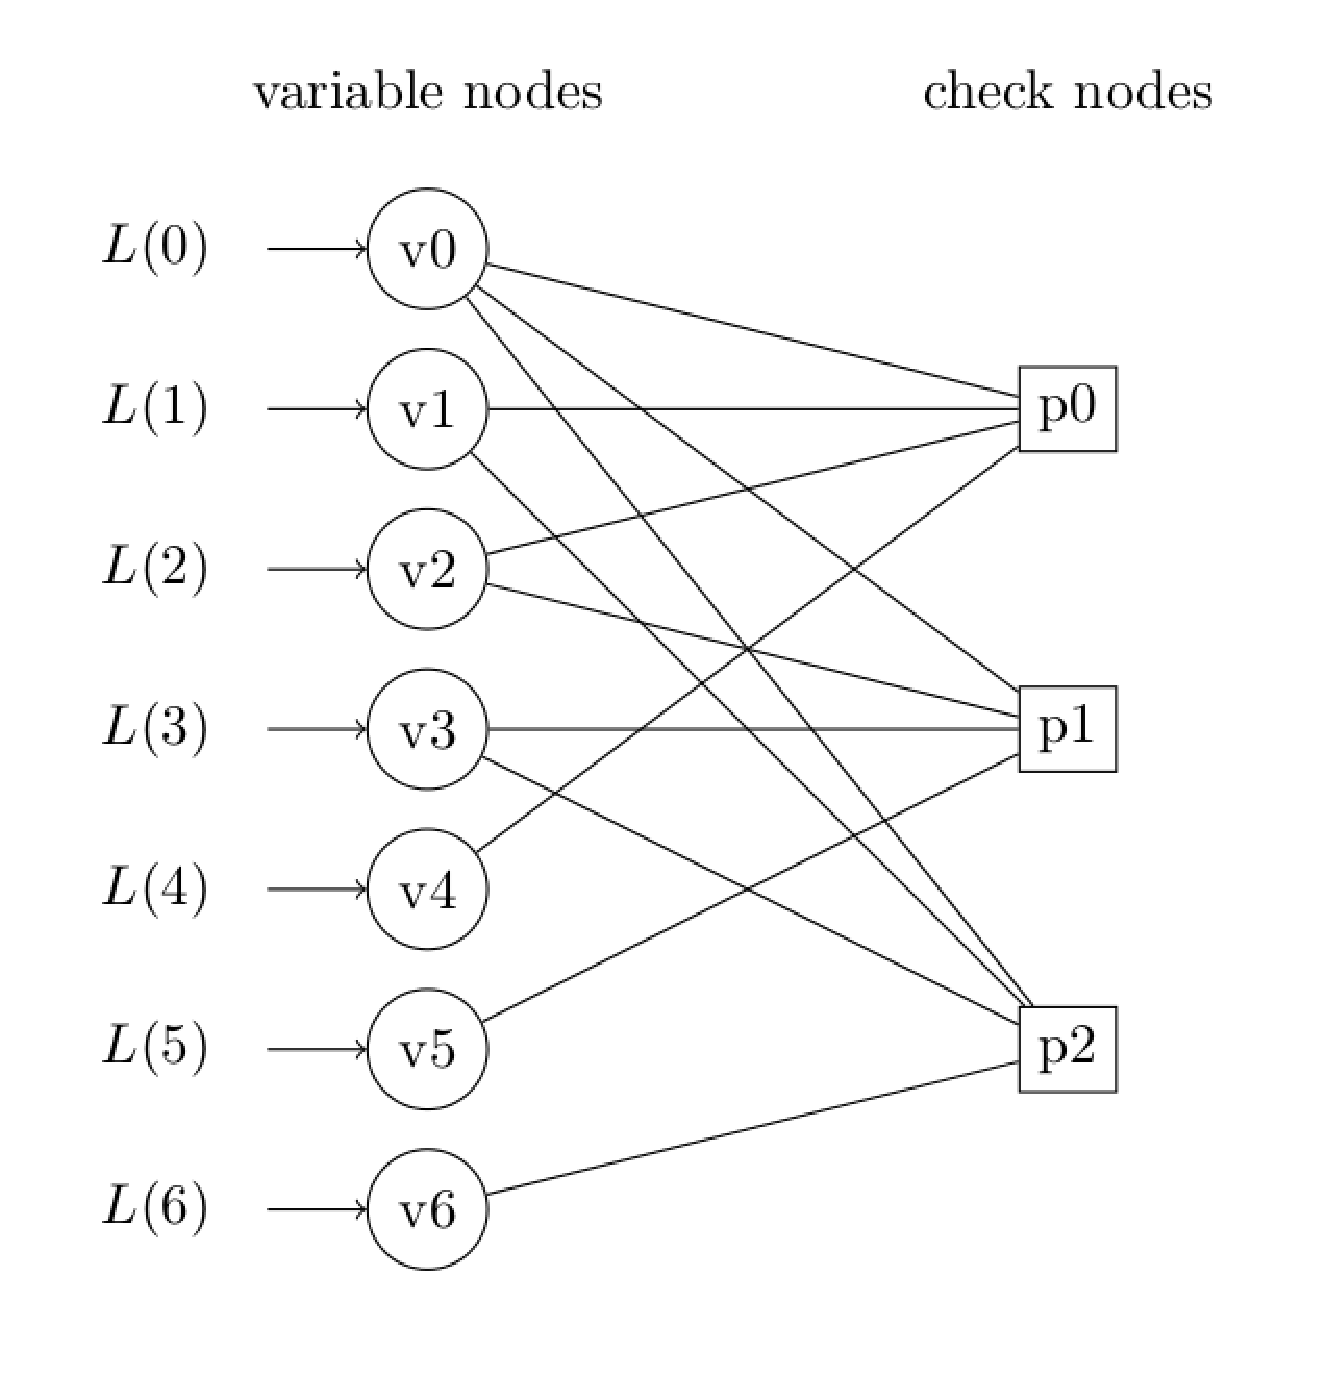
\includegraphics[width=\columnwidth]{./figs/tanner}
\caption{Tanner Graph Representation for (7,4) Hamming parity check matrix}
\label{fig:tanner}
\end{center}
\end{figure}
Encoding can be carried out by using 
\begin{align}
H &\times c^T =0 \\
 \begin{bmatrix} 
1 & 1 & 1 & 0 & 1 & 0 & 0 \\
1 & 0 & 1 & 1 & 0 & 1 & 0 \\
1 & 1 & 0 & 1 & 0 & 0 & 1 
\end{bmatrix} &  \begin{bmatrix} 
m_0\\
m_1\\
m_2\\
m_3 \\
p_0 \\
p_1\\
p_2
\end{bmatrix} = 0
\end{align}
solving we get
\begin{align}
p_0 &= m_0 \oplus m_1 \oplus m_2 \\
p_1 &= m_0 \oplus m_2 \oplus m_3 \\
p_2 &= m_0 \oplus m_1 \oplus m_3 
\end{align}
This is called Systematic Encoding.i.e Encoder will ensures information bits followed by parity bits.
\section{Decoding}
\subsection{Useful Calculations for proceeding LDPC Decoding }
\begin{enumerate}
\item Calculation of Input Channel Log Likelihood Ratio LLR 
\begin{align}
L(x_j)&=\log \brak{\frac{Pr(x_j=1|y)}{Pr(x_j=-1|y)}} \quad X=1-2c\\
&= \log \brak{\frac{f(y|x_j=1)Pr(x_j=1)}{f(y|x_j=-1)Pr(x_j=-1)}} \\
&= \log \brak{\frac{\frac{1}{\sqrt{2\pi\sigma^2}}e^{\frac{-(y_j-1)^2}{2\sigma^2}}}{\frac{1}{\sqrt{2\pi\sigma^2}}e ^{\frac{-(y_j+1)^2}{2\sigma^2}}} } \\
&=\log \brak{e^{\frac{2y_j}{\sigma^2}}} \\
L(x_j)&= \frac{2y_j}{\sigma^2} \label{eq :li}
\end{align}
\item Check Node Operation : \\
Lets assume that we have initilized all LLR values to variable nodes and we sent to check nodes. ${V_j}$ represents all the variable nodes which are connected to $j^{th}$ check node. Using the min-sum approximation\cite{minsum}, the message from  $j^{th}$ check node to  $i^{th}$ variable node given by,
\begin{figure}[!ht]
\begin{center}
%\begin{tikzpicture}
%    \node[shape=circle,draw=black] (v4) at (0,3) {v4};
%
%    \node[shape=circle,draw=black] (v2) at (0,4) {v2};
%    \node[shape=circle,draw=black] (v1) at (0,5) {v1};
%    \node[shape=circle,draw=black] (v0) at (0,6) {v0};
%
%    \node[shape=rectangle,draw=black] (p0) at (3,5) {p0};
%
%\path [<-] (v0) edge node[left] {} (p0);
%
%\path [->] (v1) edge node[left] {} (p0);
%
%\path [->] (v2) edge node[left] {} (p0);
%
%\path [->] (v4) edge node[left] {} (p0);
%
%
%
%\path [->] (-1,3) edge node[left] {} (v4);
%\path [->] (-1,4) edge node[left] {} (v2);
%\path [->] (-1,5) edge node[left] {} (v1);
%\path [->] (-1,6) edge node[left] {} (v0);
%
%
%\node[] at (-1.7,3) {$L(4)$};
%\node[] at (-1.7,4) {$L(2)$};
%\node[] at (-1.7,5) {$L(1)$};
%\node[] at (-1.7,6) {$L(0)$};
%
%
%\end{tikzpicture}
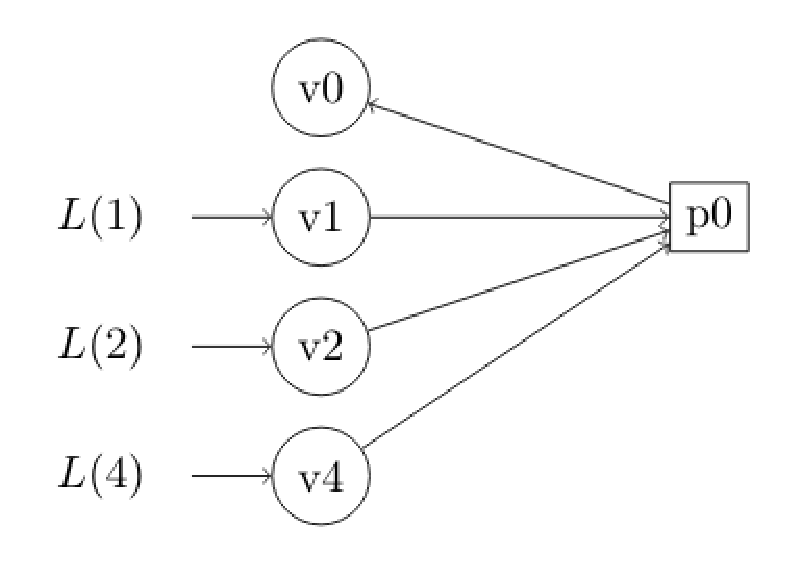
\includegraphics[width=\columnwidth]{./figs/checkope}
\end{center}
\caption{Check node operation}
\label{fig : check}
\end{figure}
since parity node equation for the first check node is $p_0=m_0+m_1+m_2+m_4$. we need to calculate
\begin{align}
L_{ext0,0} &= \log \brak{\frac{Pr(x_0 =0 | y_1,y_2,y_4)}{Pr(x_0 =1| y_1,y_2,y_4)}}
\end{align}
Defining,
\begin{align}
L_1 &= \log \brak{\frac{Pr(x_1 =0 | y_1)}{Pr(x_1 =1| y_1)}} = \log \brak{\frac{p_1}{1-p_1}} \\
L_2 &= \log \brak{\frac{Pr(x_2 =0 | y_2)}{Pr(x_2 =1| y_2)}}=\log \brak{\frac{p_2}{1-p_2}} \\
L_4 &= \log \brak{\frac{Pr(x_4 =0 | y_4)}{Pr(x_4 =1| y_4)}}= \log \brak{\frac{p_4}{1-p_4}} \\
\end{align}
\begin{table}[!ht]
\begin{center}
{\tiny
%%%%%%%%%%%%%%%%%%%%%%%%%%%%%%%%%%%%%%%%%%%%%%%%%%%%%%%%%%%%%%%%%%%%%%
%%                                                                  %%
%%  This is the header of a LaTeX2e file exported from Gnumeric.    %%
%%                                                                  %%
%%  This file can be compiled as it stands or included in another   %%
%%  LaTeX document. The table is based on the longtable package so  %%
%%  the longtable options (headers, footers...) can be set in the   %%
%%  preamble section below (see PRAMBLE).                           %%
%%                                                                  %%
%%  To include the file in another, the following two lines must be %%
%%  in the including file:                                          %%
%%        \def\inputGnumericTable{}                                 %%
%%  at the beginning of the file and:                               %%
%%        \input{name-of-this-file.tex}                             %%
%%  where the table is to be placed. Note also that the including   %%
%%  file must use the following packages for the table to be        %%
%%  rendered correctly:                                             %%
%%    \usepackage[latin1]{inputenc}                                 %%
%%    \usepackage{color}                                            %%
%%    \usepackage{array}                                            %%
%%    \usepackage{longtable}                                        %%
%%    \usepackage{calc}                                             %%
%%    \usepackage{multirow}                                         %%
%%    \usepackage{hhline}                                           %%
%%    \usepackage{ifthen}                                           %%
%%  optionally (for landscape tables embedded in another document): %%
%%    \usepackage{lscape}                                           %%
%%                                                                  %%
%%%%%%%%%%%%%%%%%%%%%%%%%%%%%%%%%%%%%%%%%%%%%%%%%%%%%%%%%%%%%%%%%%%%%%



%%  This section checks if we are begin input into another file or  %%
%%  the file will be compiled alone. First use a macro taken from   %%
%%  the TeXbook ex 7.7 (suggestion of Han-Wen Nienhuys).            %%
\def\ifundefined#1{\expandafter\ifx\csname#1\endcsname\relax}


%%  Check for the \def token for inputed files. If it is not        %%
%%  defined, the file will be processed as a standalone and the     %%
%%  preamble will be used.                                          %%
\ifundefined{inputGnumericTable}

%%  We must be able to close or not the document at the end.        %%
	\def\gnumericTableEnd{\end{document}}


%%%%%%%%%%%%%%%%%%%%%%%%%%%%%%%%%%%%%%%%%%%%%%%%%%%%%%%%%%%%%%%%%%%%%%
%%                                                                  %%
%%  This is the PREAMBLE. Change these values to get the right      %%
%%  paper size and other niceties.                                  %%
%%                                                                  %%
%%%%%%%%%%%%%%%%%%%%%%%%%%%%%%%%%%%%%%%%%%%%%%%%%%%%%%%%%%%%%%%%%%%%%%

	\documentclass[12pt%
			  %,landscape%
                    ]{report}
       \usepackage[latin1]{inputenc}
       \usepackage{fullpage}
       \usepackage{color}
       \usepackage{array}
       \usepackage{longtable}
       \usepackage{calc}
       \usepackage{multirow}
       \usepackage{hhline}
       \usepackage{ifthen}

	\begin{document}


%%  End of the preamble for the standalone. The next section is for %%
%%  documents which are included into other LaTeX2e files.          %%
\else

%%  We are not a stand alone document. For a regular table, we will %%
%%  have no preamble and only define the closing to mean nothing.   %%
    \def\gnumericTableEnd{}

%%  If we want landscape mode in an embedded document, comment out  %%
%%  the line above and uncomment the two below. The table will      %%
%%  begin on a new page and run in landscape mode.                  %%
%       \def\gnumericTableEnd{\end{landscape}}
%       \begin{landscape}


%%  End of the else clause for this file being \input.              %%
\fi

%%%%%%%%%%%%%%%%%%%%%%%%%%%%%%%%%%%%%%%%%%%%%%%%%%%%%%%%%%%%%%%%%%%%%%
%%                                                                  %%
%%  The rest is the gnumeric table, except for the closing          %%
%%  statement. Changes below will alter the table's appearance.     %%
%%                                                                  %%
%%%%%%%%%%%%%%%%%%%%%%%%%%%%%%%%%%%%%%%%%%%%%%%%%%%%%%%%%%%%%%%%%%%%%%

\providecommand{\gnumericmathit}[1]{#1} 
%%  Uncomment the next line if you would like your numbers to be in %%
%%  italics if they are italizised in the gnumeric table.           %%
%\renewcommand{\gnumericmathit}[1]{\mathit{#1}}
\providecommand{\gnumericPB}[1]%
{\let\gnumericTemp=\\#1\let\\=\gnumericTemp\hspace{0pt}}
 \ifundefined{gnumericTableWidthDefined}
        \newlength{\gnumericTableWidth}
        \newlength{\gnumericTableWidthComplete}
        \newlength{\gnumericMultiRowLength}
        \global\def\gnumericTableWidthDefined{}
 \fi
%% The following setting protects this code from babel shorthands.  %%
 \ifthenelse{\isundefined{\languageshorthands}}{}{\languageshorthands{english}}
%%  The default table format retains the relative column widths of  %%
%%  gnumeric. They can easily be changed to c, r or l. In that case %%
%%  you may want to comment out the next line and uncomment the one %%
%%  thereafter                                                      %%
\providecommand\gnumbox{\makebox[0pt]}
%%\providecommand\gnumbox[1][]{\makebox}

%% to adjust positions in multirow situations                       %%
\setlength{\bigstrutjot}{\jot}
\setlength{\extrarowheight}{\doublerulesep}

%%  The \setlongtables command keeps column widths the same across  %%
%%  pages. Simply comment out next line for varying column widths.  %%
\setlongtables

\setlength\gnumericTableWidth{%
	53pt+%
	53pt+%
	53pt+%
	53pt+%
0pt}
\def\gumericNumCols{4}
\setlength\gnumericTableWidthComplete{\gnumericTableWidth+%
         \tabcolsep*\gumericNumCols*2+\arrayrulewidth*\gumericNumCols}
\ifthenelse{\lengthtest{\gnumericTableWidthComplete > \linewidth}}%
         {\def\gnumericScale{\ratio{\linewidth-%
                        \tabcolsep*\gumericNumCols*2-%
                        \arrayrulewidth*\gumericNumCols}%
{\gnumericTableWidth}}}%
{\def\gnumericScale{1}}

%%%%%%%%%%%%%%%%%%%%%%%%%%%%%%%%%%%%%%%%%%%%%%%%%%%%%%%%%%%%%%%%%%%%%%
%%                                                                  %%
%% The following are the widths of the various columns. We are      %%
%% defining them here because then they are easier to change.       %%
%% Depending on the cell formats we may use them more than once.    %%
%%                                                                  %%
%%%%%%%%%%%%%%%%%%%%%%%%%%%%%%%%%%%%%%%%%%%%%%%%%%%%%%%%%%%%%%%%%%%%%%

\ifthenelse{\isundefined{\gnumericColA}}{\newlength{\gnumericColA}}{}\settowidth{\gnumericColA}{\begin{tabular}{@{}p{53pt*\gnumericScale}@{}}x\end{tabular}}
\ifthenelse{\isundefined{\gnumericColB}}{\newlength{\gnumericColB}}{}\settowidth{\gnumericColB}{\begin{tabular}{@{}p{53pt*\gnumericScale}@{}}x\end{tabular}}
\ifthenelse{\isundefined{\gnumericColC}}{\newlength{\gnumericColC}}{}\settowidth{\gnumericColC}{\begin{tabular}{@{}p{53pt*\gnumericScale}@{}}x\end{tabular}}
\ifthenelse{\isundefined{\gnumericColD}}{\newlength{\gnumericColD}}{}\settowidth{\gnumericColD}{\begin{tabular}{@{}p{53pt*\gnumericScale}@{}}x\end{tabular}}

\begin{tabular}[c]{%
	b{\gnumericColA}%
	b{\gnumericColB}%
	b{\gnumericColC}%
	b{\gnumericColD}%
	}

%%%%%%%%%%%%%%%%%%%%%%%%%%%%%%%%%%%%%%%%%%%%%%%%%%%%%%%%%%%%%%%%%%%%%%
%%  The longtable options. (Caption, headers... see Goosens, p.124) %%
%	\caption{The Table Caption.}             \\	%
% \hline	% Across the top of the table.
%%  The rest of these options are table rows which are placed on    %%
%%  the first, last or every page. Use \multicolumn if you want.    %%

%%  Header for the first page.                                      %%
%	\multicolumn{4}{c}{The First Header} \\ \hline 
%	\multicolumn{1}{c}{colTag}	%Column 1
%	&\multicolumn{1}{c}{colTag}	%Column 2
%	&\multicolumn{1}{c}{colTag}	%Column 3
%	&\multicolumn{1}{c}{colTag}	\\ \hline %Last column
%	\endfirsthead

%%  The running header definition.                                  %%
%	\hline
%	\multicolumn{4}{l}{\ldots\small\slshape continued} \\ \hline
%	\multicolumn{1}{c}{colTag}	%Column 1
%	&\multicolumn{1}{c}{colTag}	%Column 2
%	&\multicolumn{1}{c}{colTag}	%Column 3
%	&\multicolumn{1}{c}{colTag}	\\ \hline %Last column
%	\endhead

%%  The running footer definition.                                  %%
%	\hline
%	\multicolumn{4}{r}{\small\slshape continued\ldots} \\
%	\endfoot

%%  The ending footer definition.                                   %%
%	\multicolumn{4}{c}{That's all folks} \\ \hline 
%	\endlastfoot
%%%%%%%%%%%%%%%%%%%%%%%%%%%%%%%%%%%%%%%%%%%%%%%%%%%%%%%%%%%%%%%%%%%%%%

\hhline{|-|-|-|-}
	 \multicolumn{1}{|p{\gnumericColA}|}%
	{\gnumericPB{\centering}\gnumbox{c0}}
	&\multicolumn{1}{p{\gnumericColB}|}%
	{\gnumericPB{\centering}\gnumbox{c1}}
	&\multicolumn{1}{p{\gnumericColC}|}%
	{\gnumericPB{\centering}\gnumbox{c2}}
	&\multicolumn{1}{p{\gnumericColD}|}%
	{\gnumericPB{\centering}\gnumbox{c4}}
\\
\hhline{|----|}
	 \multicolumn{1}{|p{\gnumericColA}|}%
	{\gnumericPB{\centering}\gnumbox{0}}
	&\multicolumn{1}{p{\gnumericColB}|}%
	{\gnumericPB{\centering}\gnumbox{0}}
	&\multicolumn{1}{p{\gnumericColC}|}%
	{\gnumericPB{\centering}\gnumbox{0}}
	&\multicolumn{1}{p{\gnumericColD}|}%
	{\gnumericPB{\centering}\gnumbox{0}}
\\
\hhline{|----|}
	 \multicolumn{1}{|p{\gnumericColA}|}%
	{\gnumericPB{\centering}\gnumbox{1}}
	&\multicolumn{1}{p{\gnumericColB}|}%
	{\gnumericPB{\centering}\gnumbox{0}}
	&\multicolumn{1}{p{\gnumericColC}|}%
	{\gnumericPB{\centering}\gnumbox{0}}
	&\multicolumn{1}{p{\gnumericColD}|}%
	{\gnumericPB{\centering}\gnumbox{1}}
\\
\hhline{|----|}
	 \multicolumn{1}{|p{\gnumericColA}|}%
	{\gnumericPB{\centering}\gnumbox{1}}
	&\multicolumn{1}{p{\gnumericColB}|}%
	{\gnumericPB{\centering}\gnumbox{0}}
	&\multicolumn{1}{p{\gnumericColC}|}%
	{\gnumericPB{\centering}\gnumbox{1}}
	&\multicolumn{1}{p{\gnumericColD}|}%
	{\gnumericPB{\centering}\gnumbox{0}}
\\
\hhline{|----|}
	 \multicolumn{1}{|p{\gnumericColA}|}%
	{\gnumericPB{\centering}\gnumbox{0}}
	&\multicolumn{1}{p{\gnumericColB}|}%
	{\gnumericPB{\centering}\gnumbox{0}}
	&\multicolumn{1}{p{\gnumericColC}|}%
	{\gnumericPB{\centering}\gnumbox{1}}
	&\multicolumn{1}{p{\gnumericColD}|}%
	{\gnumericPB{\centering}\gnumbox{1}}
\\
\hhline{|----|}
	 \multicolumn{1}{|p{\gnumericColA}|}%
	{\gnumericPB{\centering}\gnumbox{1}}
	&\multicolumn{1}{p{\gnumericColB}|}%
	{\gnumericPB{\centering}\gnumbox{1}}
	&\multicolumn{1}{p{\gnumericColC}|}%
	{\gnumericPB{\centering}\gnumbox{0}}
	&\multicolumn{1}{p{\gnumericColD}|}%
	{\gnumericPB{\centering}\gnumbox{0}}
\\
\hhline{|----|}
	 \multicolumn{1}{|p{\gnumericColA}|}%
	{\gnumericPB{\centering}\gnumbox{0}}
	&\multicolumn{1}{p{\gnumericColB}|}%
	{\gnumericPB{\centering}\gnumbox{1}}
	&\multicolumn{1}{p{\gnumericColC}|}%
	{\gnumericPB{\centering}\gnumbox{0}}
	&\multicolumn{1}{p{\gnumericColD}|}%
	{\gnumericPB{\centering}\gnumbox{1}}
\\
\hhline{|----|}
	 \multicolumn{1}{|p{\gnumericColA}|}%
	{\gnumericPB{\centering}\gnumbox{0}}
	&\multicolumn{1}{p{\gnumericColB}|}%
	{\gnumericPB{\centering}\gnumbox{1}}
	&\multicolumn{1}{p{\gnumericColC}|}%
	{\gnumericPB{\centering}\gnumbox{1}}
	&\multicolumn{1}{p{\gnumericColD}|}%
	{\gnumericPB{\centering}\gnumbox{0}}
\\
\hhline{|----|}
	 \multicolumn{1}{|p{\gnumericColA}|}%
	{\gnumericPB{\centering}\gnumbox{1}}
	&\multicolumn{1}{p{\gnumericColB}|}%
	{\gnumericPB{\centering}\gnumbox{1}}
	&\multicolumn{1}{p{\gnumericColC}|}%
	{\gnumericPB{\centering}\gnumbox{1}}
	&\multicolumn{1}{p{\gnumericColD}|}%
	{\gnumericPB{\centering}\gnumbox{1}}
\\
\hhline{|-|-|-|-|}
\end{tabular}

\ifthenelse{\isundefined{\languageshorthands}}{}{\languageshorthands{\languagename}}
\gnumericTableEnd

}
\end{center}
\caption{Probability of a varibale node from other check nodes}
\label{table:type}
\end{table}
Using Table. \ref{table:type} we can find the 
\begin{equation}
p_0=Pr(c_0=0|c_1,c_2,c_4)
\end{equation}
\begin{align*}
p_0 &= p_1p_2p_4 + p_1(1-p_2)(1-p_4)\\
&+(1-p_1)p_2(1-p_4)
+(1-p_1)(1-p_2)p_4\\
1-p_0 &=p_1p_2(1-p_4) + p_1(1-p_2)p_4\\
&+(1-p_1)p_2p_4+(1-p_1)(1-p_2)(1-p_4)\\
\end{align*}
by rearranging above equations,
\begin{equation}
p_0 - (1-p_0) = p_1 -(1-p_1) + p_2 - (1-p_2) + p_4 -(1- p_4)
\end{equation}
%\begin{equation}\label{eq:sub}
%\log \brak{\frac{1-\frac{1-p_0}{p_0}}{1+\frac{1-p_0}{p_0}}}
%\end{equation}

Where $p_i$ is the probability. getting message from check to variable node by taking all variable node informations.
\begin{align}
\frac{1-\frac{1-p_0}{p_0}}{1+\frac{1-p_0}{p_0}} & = \frac{1-\frac{1-p_1}{p_1}}{1+\frac{1-p_1}{p_1}} \times \frac{1-\frac{1-p_2}{p_2}}{1+\frac{1-p_2}{p_2}} \times \frac{1-\frac{1-p_4}{p_4}}{1+\frac{1-p_4}{p_4}}\\
\frac{1-e^{-L_{ext0,0}}}{1+e^{-L_{ext0,0}}} &=\frac{1-e^{-L_{1}}}{1+e^{-L_{1}}}\times \frac{1-e^{-L_{2}}}{1+e^{-L_{2}}} \times \frac{1-e^{-L_{4}}}{1+e^{-L_{4}}}\\ \nonumber
-\tanh \brak{\frac{L_{ext0,0}}{2}}& =\brak{-\tanh \brak{\frac{L_{1}}{2}}}\brak{-\tanh \brak{\frac{L_{2}}{2}}}\\
&\brak{ -\tanh \brak{\frac{L_{4}}{2}} }
\end{align}
\begin{align}
\tanh \brak{\frac{L_{ext0,0}}{2}} &=\sbrak{\prod_{k \in V_j \setminus i}\alpha_{k,0}}\sbrak{\prod_{k \in V_j \setminus i} \tanh \brak{\frac{\beta_{k,0}}{2}}}\\
L_{ext0,0}  &=\brak{\prod_{k \in V_j \setminus i}\alpha_{k,0}}2 tanh^{-1}\brak{\prod_{k \in V_j \setminus i} \tanh \brak{\frac{\beta_{k,0}}{2}}}\\
&=\brak{\prod_{k \in V_j \setminus i}\alpha_{k,0}}\\
&2 tanh^{-1}\log^- \log\brak{\prod_{k \in V_j \setminus i} \tanh \brak{\frac{\beta_{k,0}}{2}}}\\
&=\brak{\prod_{k \in V_j \setminus i}\alpha_{k,0}}\\
&2 tanh^{-1}\log^{-1}\brak{\sum_{k \in V_j \setminus i} \log \tanh \brak{\frac{\beta_{k,0}}{2}}}\\
L_{ext0,0}&=\brak{\prod_{k \in V_j \setminus i}\alpha_{k,0}} f\brak{\sum_{k \in V_j \setminus i}f\brak{\beta_{k,0}}} \label{eq:main}
\end{align}
Where,
\begin{align}
\alpha_{k,j}&=sign(L_{k,j})\\
\beta_{k,j}&=\abs{L_{k,j}}\\
f(x)&= - \log \brak{\tanh{\frac{x}{2}}}
\end{align}
 \begin{figure}[!ht]
\begin{center}
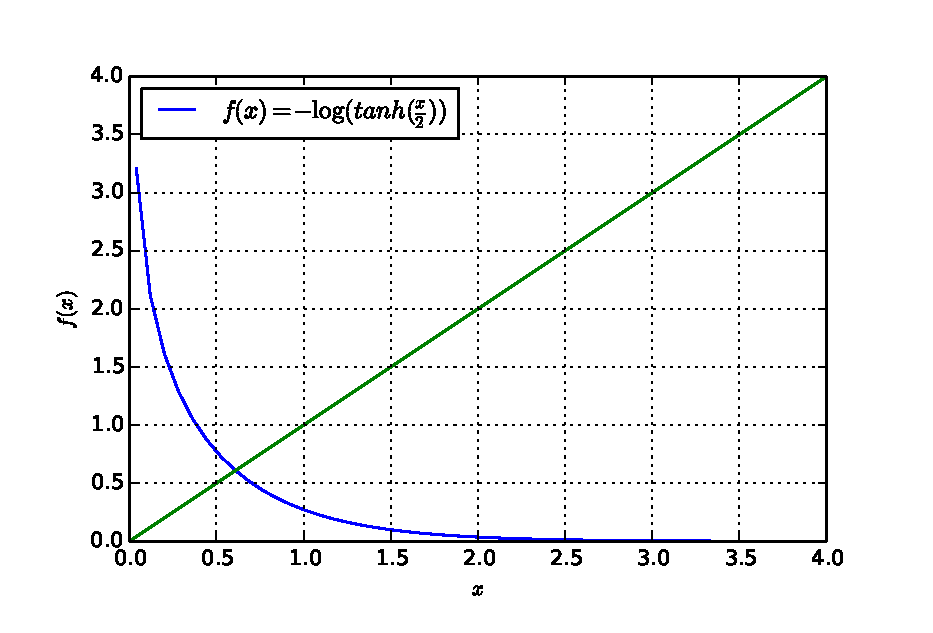
\includegraphics[width=\columnwidth]{./figs/fxgraph}
\caption{Plot of function $f(x)$}
\label{fig : fx}
\end{center}
\end{figure}
Using the Fig \ref{fig : fx}, we can approximate the above equation as, given by minimum sum approximation \cite{minsum} 
\begin{align}
f\brak{\sum_{k \in V_j \setminus i}f\brak{\beta_{k,0}}} &\approx f\brak{f\brak{\min_{k \in V_j \setminus i}\brak{\beta_{k,0}}}}\\
&=\min_{k \in V_j \setminus i}\brak{\beta_{k,0}} \label{eq: minsumapp}
\end{align}
Combining \eqref{eq: minsumapp} in \eqref{eq:main},
\begin{align}
L(r_{j=0,i=0}) &=\brak{\prod_{k \in V_j \setminus i}\alpha_{k,0}} \brak{\min_{k \in V_j \setminus i}\brak{\beta_{k,0}}} \label{eq:rji}
\end{align}
%
\item Variable Node Operation :\\
Let ${C_i}$ denotes all the check nodes connected to $i^{th}$ variable node. The message from $i^{th}$ variable node to  $j^{th}$ check node given by,
\begin{figure}[!ht]
\begin{center}
%\begin{tikzpicture}
%
%    
%    \node[shape=circle,draw=black] (v0) at (0,3) {v0};
%
%    
%
%
%    \node[shape=rectangle,draw=black] (p0) at (2,4) {p0};
%    \node[shape=rectangle,draw=black] (p1) at (2,3) {p1};
%    \node[shape=rectangle,draw=black] (p2) at (2,2) {p2};
%
%\path [->] (v0) edge node[left] {} (p0);
%\path [<-] (v0) edge node[left] {} (p1);
%\path [<-] (v0) edge node[left] {} (p2);
%
%
%\path [->] (-1,3) edge node[left] {} (v0);
%
%\node[] at (-1.4,3) {$L(0)$};
%
%\end{tikzpicture}
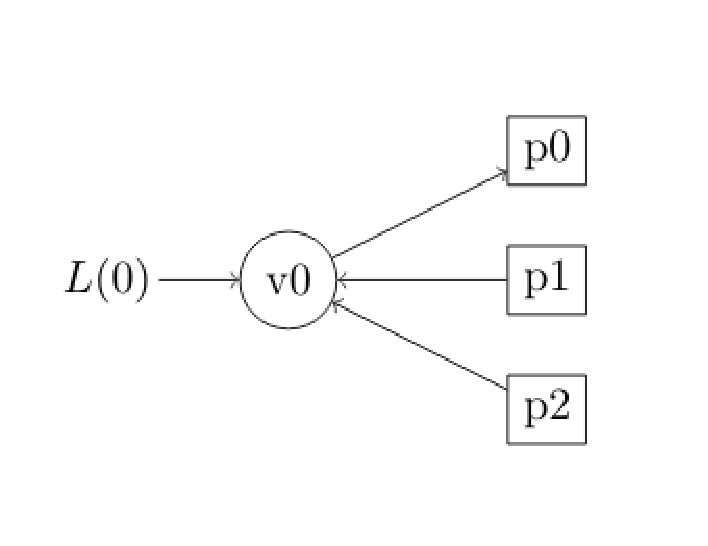
\includegraphics[width=\columnwidth]{./figs/varope}
\end{center}
\caption{Variable node operation}
\label{fig : var}
\end{figure}
\begin{align}
L(q_{i=0,j=0})&=\log \brak{\frac{Pr(x_j=1|y_0,y_1,y_2)}{Pr(x_j=-1|y_0,y_1,y_2)}} \quad X=1-2c\\
&= \log \brak{\frac{f(y_0,y1,y_2|x_j=1)Pr(x_j=1)}{f(y_0,y_1,y_2|x_j=-1)Pr(x_j=-1)}} \\
&= \log \brak{\frac{\brak{\frac{1}{\sqrt{2\pi\sigma^2}}}^3e^{\frac{-(y_0-1)^2}{2\sigma^2}}e^{\frac{-(y_1-1)^2}{2\sigma^2}}e^{\frac{-(y_2-1)^2}{2\sigma^2}}}{\brak{\frac{1}{\sqrt{2\pi\sigma^2}}}^3e ^{\frac{-(y_0+1)^2}{2\sigma^2}}e ^{\frac{-(y_1+1)^2}{2\sigma^2}}e ^{\frac{-(y_2+1)^2}{2\sigma^2}} }  } \\
&=\log \brak{e^{\frac{2(y_0+y_1+y_2)}{\sigma^2}}} \\
L(q_{i=0,j=0})&= \frac{2(y_0+y_1+y_2)}{\sigma^2}=L(x_i)+\sum_{k \in C_i\setminus j} L(r_{ki}) \label{eq: qij}
\end{align}
\end{enumerate}

\subsection{Message Passing Algorithm using min-sum Approximation}
Transmitted frames = N, Total number of bits = N $\times$ 7 and Total number of information bits = N $\times$ 4.
For Each Frame,
\begin{enumerate}
\item Initialize $L(q_{ij})$ using \eqref{eq :li} for all $i,j$ for which $h_{ij}=1$ with channel LLR's.
\item Update $\cbrak{L(r_{ji})}$ using \eqref{eq:rji}
\item Update $\cbrak{L(q_{ji})}$ using \eqref{eq: qij}.
\item Update $\cbrak{L(V_i)}$ using,
\begin{equation}
L(V_i)=L(x_i)+\sum_{k \in C_i} L(r_{ki}) \quad i=0,\dots,6.
\end{equation}
\item Proceed to step 2.\\
After maximum specified iterations,

\end{enumerate}
Decoding can be done using,
\begin{equation}
\hat{c_i} = \begin{cases}
1 & L(V_i) < 0\\
0 & else
\end{cases}
\end{equation}
%
\section{Results}
For frames N=10000.
 \begin{figure}[!ht]
\begin{center}
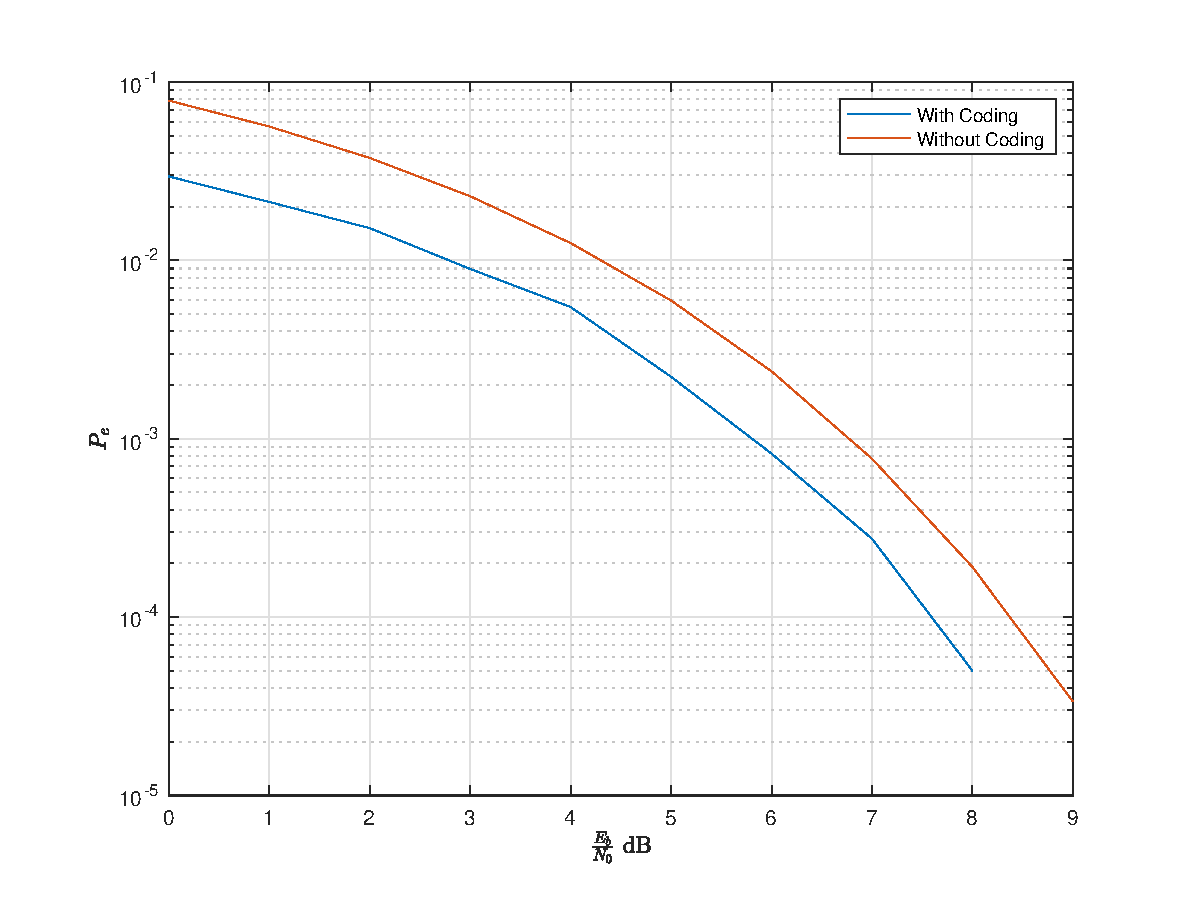
\includegraphics[width=\columnwidth]{./figs/ber}
\caption{SNR vs BER curves using LDPC channel coding and no channel coding}
\label{fig : ber}
\end{center}
\end{figure}
Fig \ref{fig : ber} Shows the Comparison of Probability error with channel coding and without channel coding. Since the parity check matrix taken was not much sparse, we are not getting near shannon limit performance. (Good sparse matrix i.e number of entries in H $<< m\times n $ )

\bibliography{IEEEabrv,ldpc.bib}
\end{document}

